\documentclass[11pt, twocolumn]{article}
\usepackage{mathptmx} % Times New Roman
\usepackage{graphicx}
\graphicspath{{figures/}}
\usepackage{amsmath,amssymb}
\usepackage{hyperref}
\usepackage{subfigure}
\usepackage{caption}
\usepackage{stfloats}
\usepackage{setspace}
\setlength{\parskip}{1em} 
\captionsetup{font=small, labelfont=bf, textfont=it, aboveskip=8pt, belowskip=2pt}
\hypersetup{colorlinks=true, urlcolor=blue, linkcolor=black, citecolor=red}
\setlength{\parindent}{0pt}

\usepackage[a4paper,top=2.5cm,bottom=2.5cm,left=2cm,right=2cm,marginparwidth=1.75cm]{geometry}

\begin{document}
\begin{titlepage}
    \centering
    \vspace*{1cm}

    {\huge \textbf{Random Variables and Random Number Generation}}

    {\huge \textit{Full Technical Report}}
    \vspace{15cm}

    {\Large Shanzi (Monica) Ran \\
    Magdalene College\\

    sr2021@cam.ac.uk\\}

    \vfill

    {\large \today}

\end{titlepage}

\section{Introduction}
    Random vairables(RV) is a key concept in statistical signal and information processing, 
    playing a significant role in various engineering applications, 
    It is  therefore important to develop efficient and reliable methods generating and presenting desired non-uniform RV distributions.
    In this report, investigations and observations of the following objectives are discussed and summarized: \newline
    \vspace{-1em}
    \begin{itemize}
        \item Generation and visualization of RV using histograms and kernel density estimation(KDE)
        \item Transformation of RV distributions using Jacobian formula
        \item Generation of non-uniform RV distributions using cumulative distribution function(CDF) and inverse CDF methods
        \item Investigation of complex RV distributions and $\alpha$-stable distribution
    \end{itemize}

\section{Results and Discussion}

\subsection{Uniform and normal RV}
\subsubsection{Histogram and KDE}

\begin{figure}[htbp]
    \centering
    \subfigure[Histogram]{
        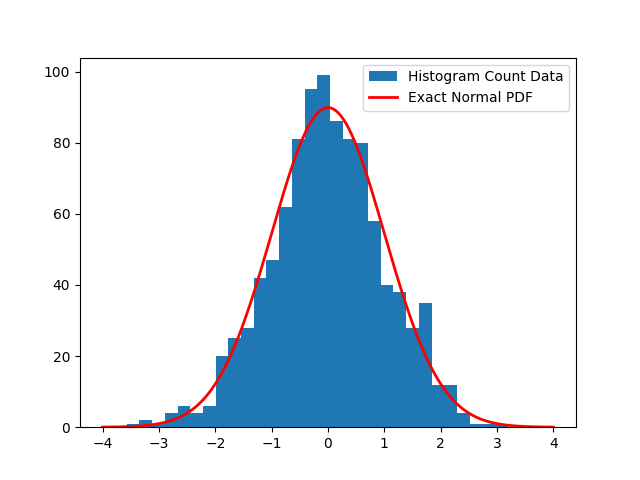
\includegraphics[width=0.225\textwidth]{q1_1}
        \label{fig:q1_1}
    }
    \subfigure[KDE]{
        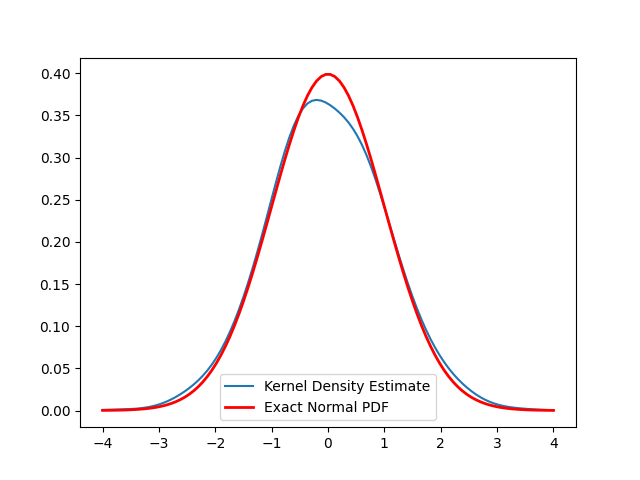
\includegraphics[width=0.225\textwidth]{q1_3}
        \label{fig:q1_3}
    }
    \caption{Histogram and KDE plot of 1000 sampled Gaussian RV $X\sim \mathcal{N}(0, 1)$}
    \label{fig:q1normal}
\end{figure}

As shown in Figure~\ref{fig:q1normal}, both histogram and KDE (with the $\mathcal{N}(0, 1)$ Gaussian kernel) produces a close approximate to the density distribution of the normal RV. 
When comparing between Fig~\ref{fig:q1_1} and Fig~\ref{fig:q1_3}, it is observed that KDE results in a more accurate approximation, which results from the smoothing of KDE, as discontinuity in histogram resulting from its discrete feature is removed.
\vspace{-1em}
\begin{figure}[htbp]
    \centering
    \subfigure[Histogram]{
        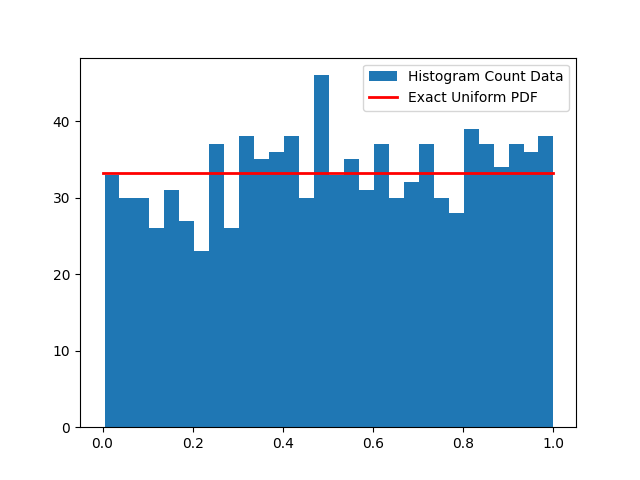
\includegraphics[width=0.225\textwidth]{q1_2}
        \label{fig:q1_2}
    }
    \subfigure[KDE (Overlaid on standard Normal)]{
        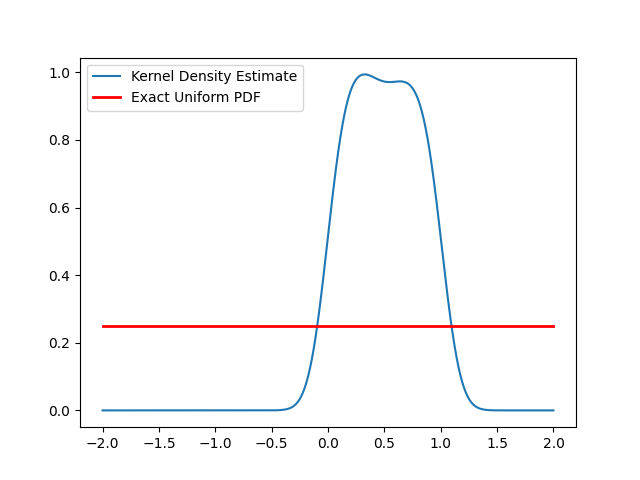
\includegraphics[width=0.225\textwidth]{q1_4}
        \label{fig:q1_4}
    }
    \caption{Histogram and KDE plot of 1000 sampled Uniform RV $X\sim\mathcal{U}(0, 1)$}
    \label{fig:q1uniform}
\end{figure}

\vspace{-1em}
In comparison, the histogram and KDE approximates for a uniform RV in Figure~\ref{fig:q1uniform} demonstrates the opposite as the histogram describes more accurately the density function of a uniform distribution because of its discontinuous property, which is less correctly depicted by KDE since the KDE smoothing removes the step changes, making the uniform distribution in Fig~\ref{fig:q1_4} appear to almost coincide a normal distribution.
This is also likely related to the specific choice of kernel
, as a uniform kernel $\mathcal{U}(0, 1)$ may suit the uniform distribution better.

\subsubsection{Multinomial distribution}
When $N$ samples of a RV with density $p(x)$ is drawn, histogramming the samples is useful in estimating the density. For histogram bin $j$ with edges $[a, b]$, the probability of a sample $x^{(i)}$ falling in this bin is:
\vspace{-0.75em}
\begin{align*}
    p_j=\int_{a}^{b}p(x)dx
\end{align*}
\vspace{-0.75em}

Since each of the $N$ samples is independent and identical distributed (iid), the joint probability of a certain outcome $(X_1=x_1, X_2=x_2, ..., X_n=x_n)$, where $X_j$ describes the number of samples falling in bin $j$, is the product of each sample falling into the corresponding bins.
Therefore, for a specific outcome of bin counts for a histogram with $n$ bins in total (when order does not matter):
\vspace{-0.75em}
\begin{align}
    \prod_{j=1}^{n}{p_j}^{x_j}
    \label{eqn1}
\end{align}


Since order does not matter, the total number of ways of reaching this outcome is given by combinactorics:
\begin{align}
    \binom{N}{x_1, ..., x_k} = \frac{N!}{x_1!x_2!...x_n!}
    \label{eqn2}
\end{align}
\vspace{-0.75em}

So probability of this distribution, equivalently the multinomial distribution probability mass function (pmf), equals $equation~\ref{eqn1}\times equation~\ref{eqn2}$:
\begin{align*}
    P(X_1=x_1, ..., X_n=x_n)=\frac{N!}{x_1!...x_n!}{{p_1}^{x_1}...{p_n}^{x_n}}
\end{align*}


\paragraph{Uniform RV with varied sample size}
For a uniform distribution, the theoretical histogram count data of each bin is identical, which can be calculated using the following equations:

\vspace{-0.75em}
\begin{align*}
    \mu&=\frac{N}{j}\\
    \sigma&=\sqrt{\frac{N}{j}(1-\frac{1}{j})}
\end{align*}

where N is total number of samples, j is total number of bins.
\begin{figure}[htbp]
    \centering
    \vspace{-1em}
    \subfigure[N=100]{
        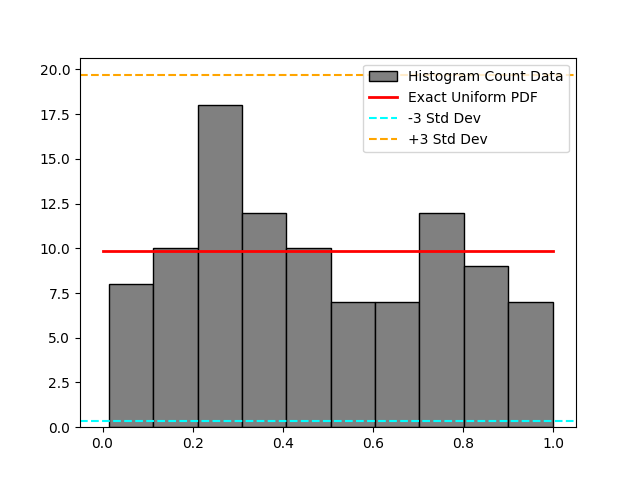
\includegraphics[width=0.5\textwidth, height=3.5cm]{q1_5_100_bin_10}
        \label{fig:q1_5_1}
    }

    \vspace{-1.1em}
    \subfigure[N=1000]{
        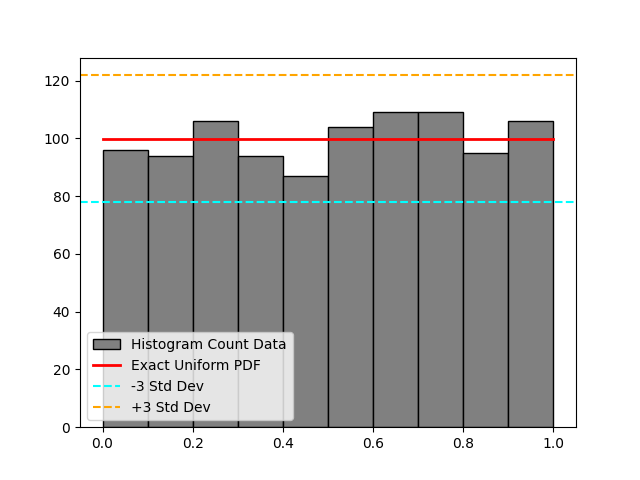
\includegraphics[width=0.5\textwidth, height=3.5cm]{q1_5_1000_bin_10}
        \label{fig:q1_5_2}
    }

    \vspace{-1.1em}
    \subfigure[N=10000]{
        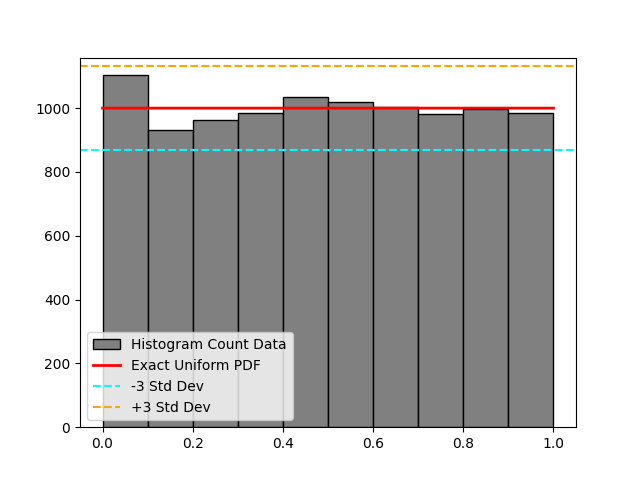
\includegraphics[width=0.5\textwidth, height=3.5cm]{q1_5_10000_bin_10}
        \label{fig:q1_5_3}
    }
    \caption{Histograms for different values of uniform RV N with theoretical $\mu$ and 3$\sigma$ lines}
    \label{fig:q1_5}
\end{figure}
\vspace{-1em}

As shown in Fig~\ref{fig:q1_5}, when sample size $N$ enlarges, the histogram count approaches to the straight line mean, and the $\pm 3\sigma$ lines are growing closer to the mean, which agrees with theoretical calculations as mean increases at $N$ and standard deviation increases slower at a rate of $\sqrt{N}$ with respect to the sample size.
Thus, the Python generated uniform distribution is accuarate, with its reliability improving for larger sample sizes which is consistent with the multinomial distribution theory.

\paragraph{Normal RV with varied sample size}
Similarly, theoretical histogram count mean and standard deviation for normal RV is calculated as below according to the multinomial distribution:
\begin{align*}
    \mu&=Np_j\\
    \sigma&=\sqrt{Np_j(1-p_j)}
\end{align*}
\vspace{-0.75em}

It should be noted that this $\mu$ and $\sigma$ differs for each of the 10 bins, with $p_j=\phi(b)-\phi(a)$ for bin $j$ with edges $[a,b]$.
\begin{figure}[htbp]
    \centering
    \vspace{-1em}
    \subfigure[N=100]{
        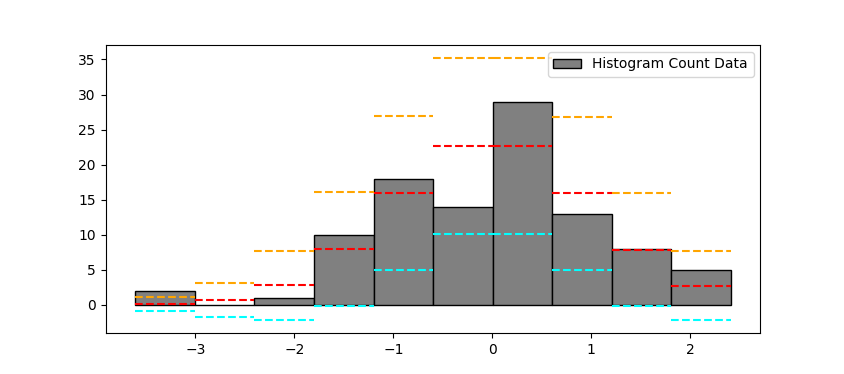
\includegraphics[width=0.5\textwidth, height=3.5cm]{q1_6_100}
        \label{fig:q1_6_1}
    }

    \vspace{-1.1em}
    \subfigure[N=1000]{
        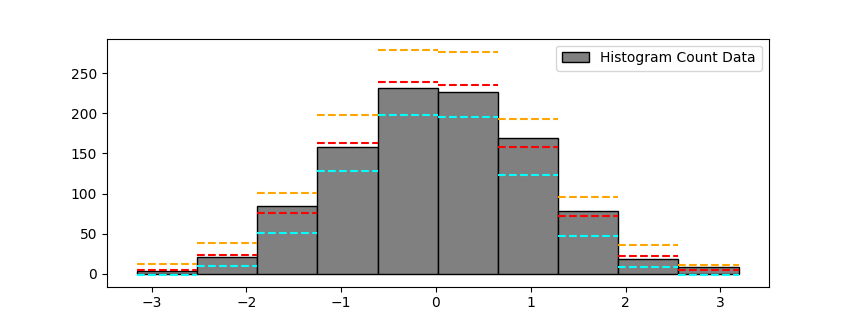
\includegraphics[width=0.5\textwidth, height=3.5cm]{q1_6_1000}
        \label{fig:q1_6_2}
    }

    \vspace{-1.1em}
    \subfigure[N=10000]{
        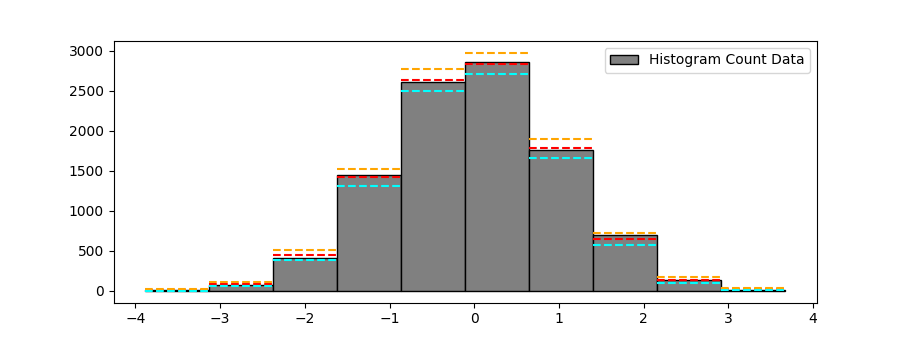
\includegraphics[width=0.5\textwidth, height=3.5cm]{q1_6_10000}
        \label{fig:q1_6_3}
    }
    \caption{Histograms for different values of normal RV N with theoretical $\mu$ and 3$\sigma$ lines}
    \label{fig:q1_6}
\end{figure}

According to Fig~\ref{fig:q1_6}, a similar trend of mean and $\pm 3\sigma$ lines approaching to be closer is observed as $N$ increases. 
Meanwhile, it is observed that when approaching the tail of the distribution where $p_j\approx 0$, since $\sigma^2\approx N{p_j}=\mu$, $\sigma\approx \sqrt{\mu}$, resulting in $-3\sigma$ lines more likely to be negative as $\mu-3\sqrt{\mu}<0$.

When $p_j$ is closer to 1, since $\sum_{j=1}^{n} p_j=1$ as probability theory requires, there is only 1 bin left on the histogram, variance is hence 0 regardless of value of $N$. 

\subsection{Functions and transformations of RV}

\subsubsection{Linear transformation $y=ax+b$}
Using the Jacobian method, density function of $y$ can be transformed from $X~\mathcal{N}(0,1)$ by function $f(x)=ax+b$ as follows:

\begin{flalign*}
    & y = f(x) = ax + b \text{, so } x = f^{-1}(y) = \frac{y - b}{a} & \\
    & \frac{dy}{dx} = a & \\
    & \begin{aligned}
        p(y) &= \frac{p(x)}{\left|\frac{dy}{dx}\right|}\Big|_{x=f^{-1}(y)} \\
             &= \frac{1}{a} p\left(\frac{y - b}{a}\right)\\
             &= \frac{1}{\sqrt{2\pi }a}exp(-\frac{1}{2}(\frac{y-b}{a})^2)
    \end{aligned} &
\end{flalign*}

which indicates that $p(y)$ is a normal density function with $\mu = b, \quad \sigma= a$.
\vspace{-1em}
\begin{figure}[h]
    \centering
    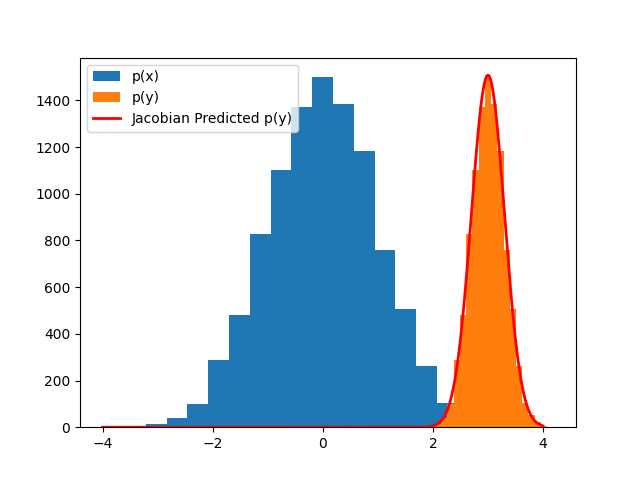
\includegraphics[width=0.45\textwidth, height=5.5cm]{q2_1}
    \caption{Sampled transformation for y=ax+b}
    \label{fig:q2_1}
\end{figure}
\vspace{-1em}
The above results is also supported by Fig~\ref{fig:q2_1} where the theoretical calculated density function of y is overlaid upon the sampled results with sample size 10000.
\vspace{-1em}

\subsubsection{Quadratic transformation $y=x^2$}

\begin{figure}[h]
    \centering
    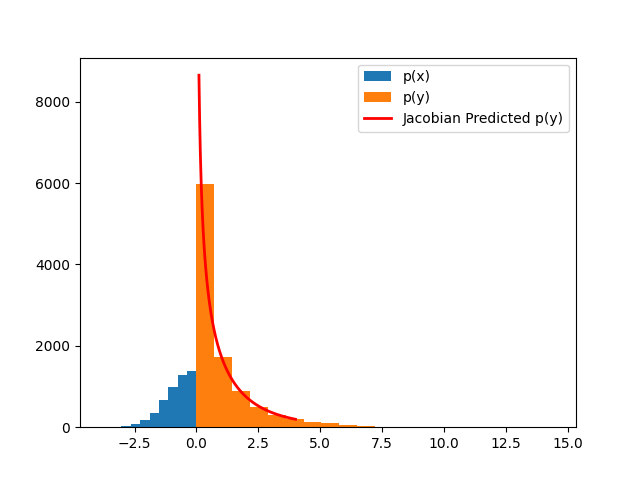
\includegraphics[width=0.45\textwidth, , height=5.5cm]{q2_2}
    \caption{Sampled transformation for $y=x^2$}
    \label{fig:q2_2}
\end{figure}
\vspace{-0.75em}
When $y=f(x)=x^2$, the Jacobian method involves summing all possible values of $f^{-1}(y)$ since this inverse function is a one-many mapping. Fig~\ref{fig:q2_2} depicts the result gathered over 10000 samples, which aligns with the calculated tranformations.

\begin{flalign*}
    & y = f(x) = x ^ 2 \text{, so } x = f^{-1}(y) = \pm \sqrt{y} \text{ , where } x_1 = \sqrt{y},\: x_2 = -\sqrt{y}& \\
    & \frac{dy}{dx} = 2x & \\
    & \begin{aligned}
        p(y) &= \sum_{k=1}^{2}\frac{p(x)}{|\frac{dy}{dx}|}\big|_{x=x_k(y)}& \\
             &= \frac{1}{\sqrt{2\pi}}exp(-\frac{y}{2})(\frac{1}{2\sqrt{y}}+|\frac{1}{2\sqrt{y}}|)& \\
             &= \frac{1}{\sqrt{2\pi y}}exp(-\frac{y}{2})
    \end{aligned} &
\end{flalign*}

\subsubsection{Trignometric transformation $y=sin(x)$}

\begin{figure}[h]
    \centering
    \subfigure[Sampled density for $y=sin(x)$]{
        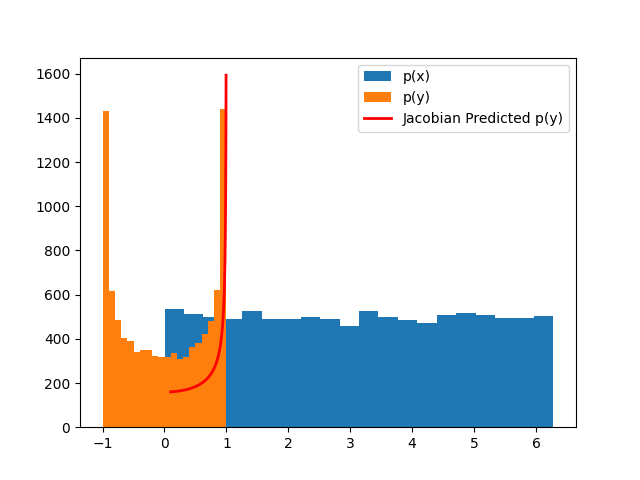
\includegraphics[width=0.45\textwidth, , height=5.5cm]{q2_3}
        \label{fig:q2_3_raw}
    }

    \vspace{-1.1em}
    \subfigure[Sampled density for $f(x)=min(sin(x),0.7)$ (zoomed in)]{
        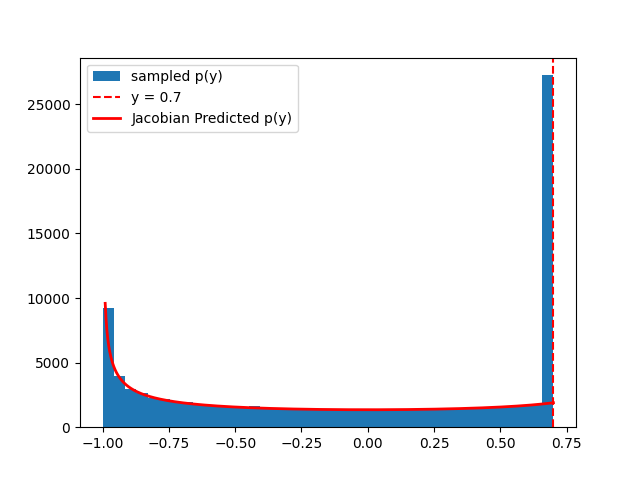
\includegraphics[width=0.45\textwidth, , height=5.5cm]{q2_3_1_with_jacobian}
        \label{fig:q2_3_jacobian}
    }
    \caption{Sampled transformation for $f(x)=sin(x)$ and $f(x)=min(sin(x),0.7)$}
    \label{fig:q1_6}
\end{figure}
\vspace{-0.75em}

For a transformation from $X~\mathcal{U}(0,2\pi)$ using $f(x)=sin(x)$:
\begin{flalign*}
    & y = f(x) = sin(x) \text{, so } x = f^{-1}(y) = sin^{-1}(y)& \\
    & \frac{dy}{dx} = cos(y) & \\
    & \begin{aligned}
        p(y) &= \frac{p(x)}{|\frac{dy}{dx}|}\big|_{x=f^{-1}(y)}& \\
             &= \frac{1}{2\pi \left|cos(sin^{-1}(y))\right|}
    \end{aligned} &
\end{flalign*}
where the absolute value is required due to the periodic feature of trigonometric transformations. This response agrees with Fig~\ref{fig:q2_3_raw}.

For a value-limited sine transformation $f(x)=min(sin(x),0.7)$, the density function is more complicated due to this "clipping":

\begin{flalign*}
    & y = f(x) = \min(\sin(x), 0.7) & \\
    & x = f^{-1}(y) = \left\{
    \begin{array}{ll}
        \sin^{-1}(y) & \text{if } -1 \leq y < 0.7, \\
        \delta(y - 0.7) & \text{if } y = 0.7, \\
    \end{array}
    \right. & \\[8pt]
    & \begin{aligned}
        p(y) &= \frac{p(x)}{\left|\frac{dy}{dx}\right|} \Big|_{x = f^{-1}(y)} \\[8pt]
             &= \left\{
                \begin{array}{ll}
                    \frac{1}{2\pi \cos(\sin^{-1}(y))} & \text{if } -1 \leq y < 0.7, \\[8pt]
                    \frac{\pi - 2\sin^{-1}(0.7)}{2\pi} \, \delta(y - 0.7) & \text{if } y = 0.7. \\
                    0 &  \text{if otherwise}
                \end{array}
             \right.
    \end{aligned} &
\end{flalign*}

The experimentally sampled data agrees with this Jacobian calcualtion and is shown in Fig~\ref{fig:q2_3_jacobian}, overlaid upon the $y=0.7$ boundary line. 

\subsection{Inverse CDF method}
\subsubsection{Generation of exponential distribution using CDF and inverse CDF}
For an exponential distribution $p(y)=exp(-y)$ for $y\geq 0$, its CDF and inverse CDF can be calculated as:
\begin{flalign*}
    & p(y) = \frac{df^{-1}(y)}{dy} = \exp(-y) & \\
    & \begin{aligned}
        \text{CDF: By definition of CDF, } F(y) &= \int_{0}^{y} p(y) \, dy &\\ 
        &= 1 - \exp(-y) &\\
    \end{aligned} &\\
    & \begin{aligned}
        \text{Inverse CDF: } &y = f(x) \; x = f^{-1}(y) &\\
                             &\text{From CDF, } x = 1 - e^{-y} &\\
                             & F^{-1}(x) = f(x) = y = -\ln(1-x) &
    \end{aligned} &\\
\end{flalign*}

\vspace{-3em}
\begin{figure}[h]
    \centering
    \subfigure[Histogram]{
        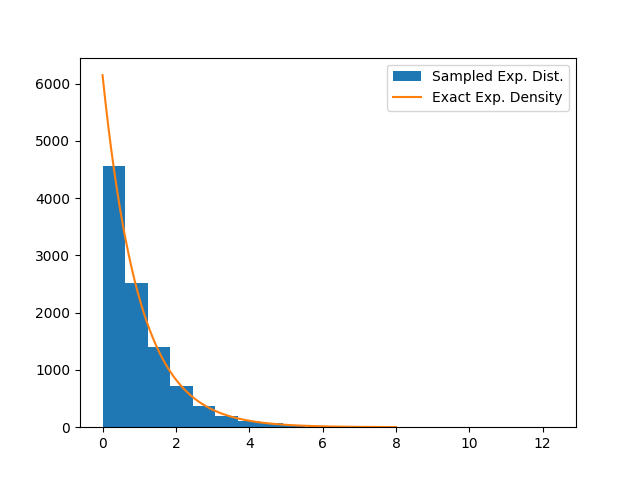
\includegraphics[width=0.5\textwidth, height=4cm]{q3_1_hist}
        \label{fig:q3_1_hist}
    }

    \vspace{-1.1em}
    \subfigure[KDE]{
        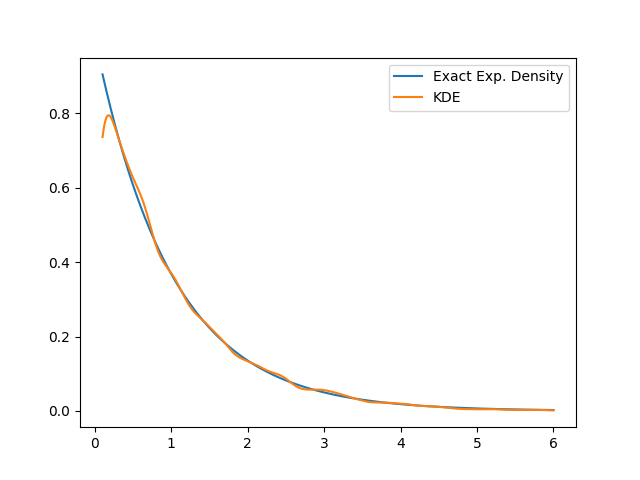
\includegraphics[width=0.5\textwidth, height=4cm]{q3_1_kde}
        \label{fig:q3_1_kde}
    }
    \caption{Sampled exponential distribution}
    \label{fig:q3_1}
\end{figure}

As demonstrated in Fig~\ref{fig:q3_1}, it can be observed that the inverse CDF method produces reliable result generating the exponential distribution that matches with both histogram and KDE graphically.

\subsubsection{Monte Carlo estimation of mean and variance of exponential distribution.}
Theoretically, an exponential distribution of $\lambda = 1$ has 
\begin{flalign*}
    & \mu = \frac{1}{lambda} = 1&\\ 
    & \sigma ^2 = \frac{1}{\lambda ^2} = 1&\\
\end{flalign*}

\vspace{-1em}
Using Monte Carlo estimates, the mean and variance of the samples of exponential distribution can be calculated as:
\begin{flalign*}
    & \mu \approx \frac{1}{N} \sum_{i=1}^{N}y^{(i)} = \hat{\mu}&\\ 
    & \sigma ^2 \approx \frac{1}{N} \sum_{i=1}^{N}(y^{(i)})^2 - \hat{\mu} ^ 2 = \hat{\sigma^2}&\\
\end{flalign*}

\begin{table}[h!]
    \centering
    \begin{tabular}{|c|c|c|}
        \hline
         & mean & variance  \\ 
        \hline
        Theoretical & 1 & 1 \\ 
        Sampled & 1.05 & 0.96 \\ 
        \hline
    \end{tabular}
    \caption{Mean and variance of theoretical and sampled distributions}
\end{table}

Comparing the calculated mean and variance from the sampled data to that of the theoretical values, it can be observed that the values are approximately close, suggesting the reliability of the Monte Carlo estimation.

\subsubsection{Proof of validity of Monte Carlo estimate}
\paragraph{Unbiased mean estimate}
\begin{flalign*}
    & \hat{\mu} = \frac{1}{N} \sum_{i=1}^{N} y_i \\
    & \text{where } y_1, ... y_n \text{are iid samples from } Y~Exp(1) \\
    & \begin{aligned}
        E[\hat{\mu}] &= E[\frac{1}{n} \sum_{i=1}^{N} y_i] \\
                     &= \frac{1}{N} E[\sum_{i=1}^{N} y_i] \\
                     &= \frac{1}{N} \sum_{i=1}^{N} E[y_i] \\
                     &= \frac{1}{N} \sum_{i=1}^{N} \mu = \mu \\
    \end{aligned} &\\
    & \text{hence } E[\hat{\mu}]=\mu \text{, the Monte Carlo mean is unbiased.}
\end{flalign*}

\paragraph{Variance of Monte Carlo mean estimator}
\begin{flalign*}
    & \begin{aligned}
        Var[\hat{\mu}] &= Var[\frac{1}{N} \sum_{i=1}^{N} y_i] \\
                       &= \frac{1}{N^2} \sum_{i=1}^{N} Var[y_i] \\
                       &= \frac{1}{N^2} (N \sigma^2) \\
                       &= \frac{\sigma^2}{N} \\
                       &= E[\hat{\mu} ^2]-E[\hat{\mu}]^2 \\
    \end{aligned} &\\
    & From above proof, E[\hat{\mu}]^2=\mu^2 =E[\mu]^2 \\
    & \begin{aligned}
        Var[\hat{\mu}] &= E[\hat{\mu} ^2]-E[\mu]^2 \\
                       &= E[\hat{\mu} ^2 - \mu^2] \propto \frac{1}{N} \\
    \end{aligned} &\\
\end{flalign*}

\subsubsection{Squared mean error $(\hat{\mu} - \mu)^2$ and Monte Carlo sample size}
\vspace{-1em}
\begin{figure}[h]
    \centering
    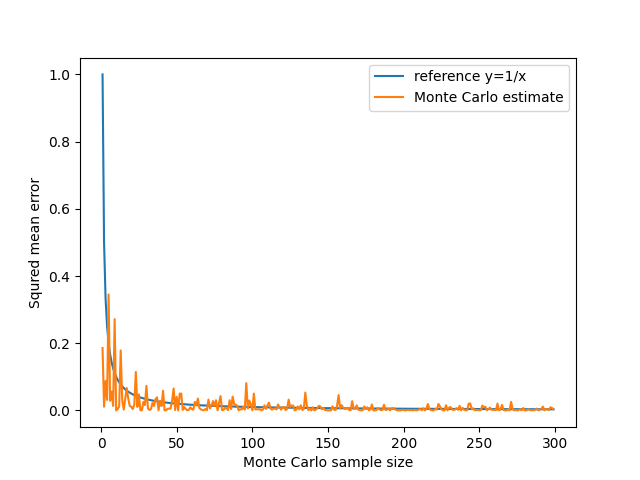
\includegraphics[width=0.45\textwidth, height=5cm]{q3_2_monte_carlo_error}
    \caption{Squared mean error with reference to $y=\sqrt(x)$}
    \label{fig:q3_m}
\end{figure}

Fig~\ref{fig:q3_m} shows that the squared error between a Monte Carlo mean estimate and the theoretical mean decays with increasing Monte Carlo sample size. 
This corresponds to a decay rate of $\frac{1}{N}$, where $N$ is the sample size taken by Monte Carlo estimator, as the trend follows the $y=\sqrt{x}$ line in the figure.


As $N$ grows, the squared mean error quickly approaches 0, further supporting the above proof that the Monte Carlo mean is unbiased.

\vspace{-0.5em}
\begin{figure*}[h]
    \centering
    % First row of 5 images
    \begin{minipage}{0.2\textwidth}
        \centering
        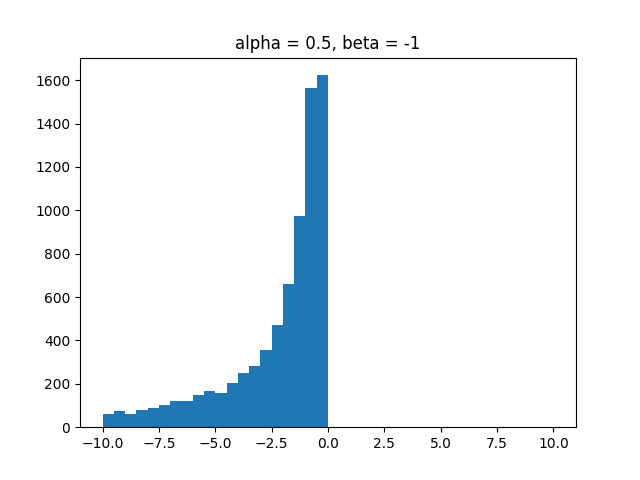
\includegraphics[width=\textwidth]{q4_1_a0.5_bn1}
    \end{minipage}%
    \begin{minipage}{0.2\textwidth}
        \centering
        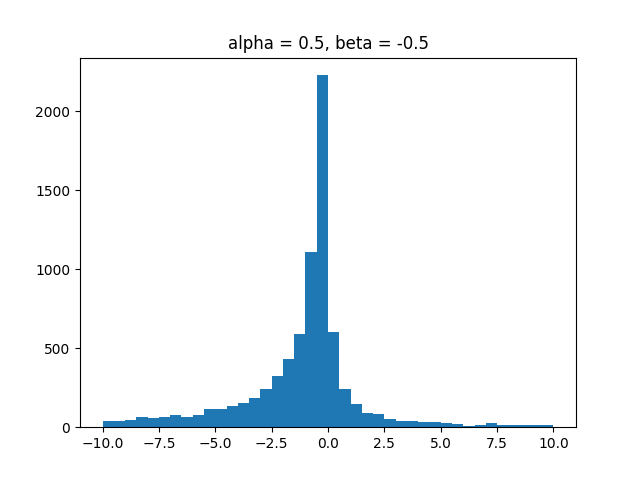
\includegraphics[width=\textwidth]{q4_1_a0.5_bn0.5}
    \end{minipage}%
    \begin{minipage}{0.2\textwidth}
        \centering
        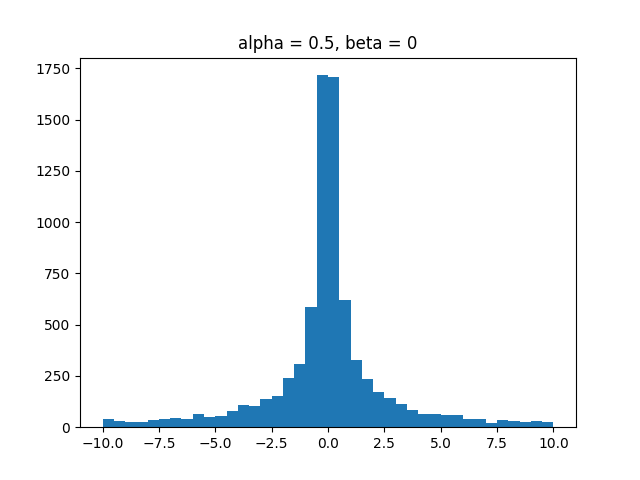
\includegraphics[width=\textwidth]{q4_1_a0.5_b0}
    \end{minipage}%
    \begin{minipage}{0.2\textwidth}
        \centering
        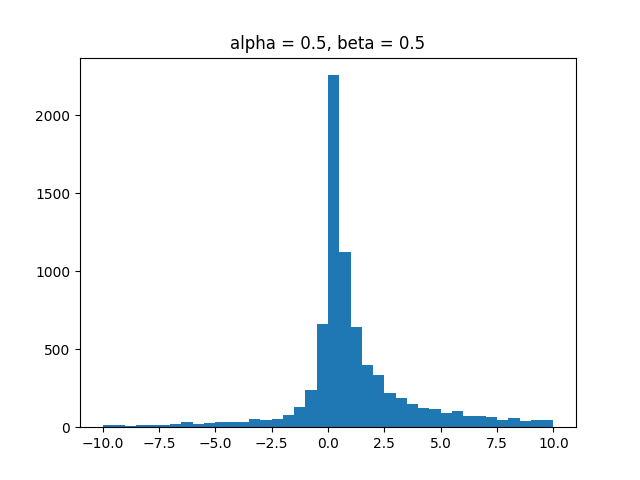
\includegraphics[width=\textwidth]{q4_1_a0.5_b0.5}
    \end{minipage}%
    \begin{minipage}{0.2\textwidth}
        \centering
        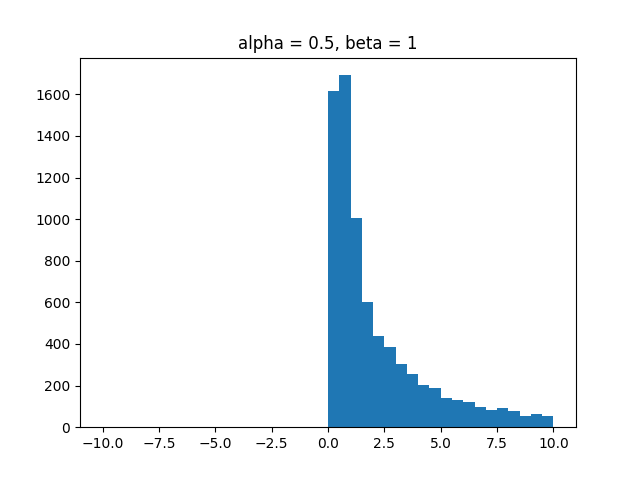
\includegraphics[width=\textwidth]{q4_1_a0.5_b1}
    \end{minipage}

    % Second row of 5 images
    \begin{minipage}{0.2\textwidth}
        \centering
        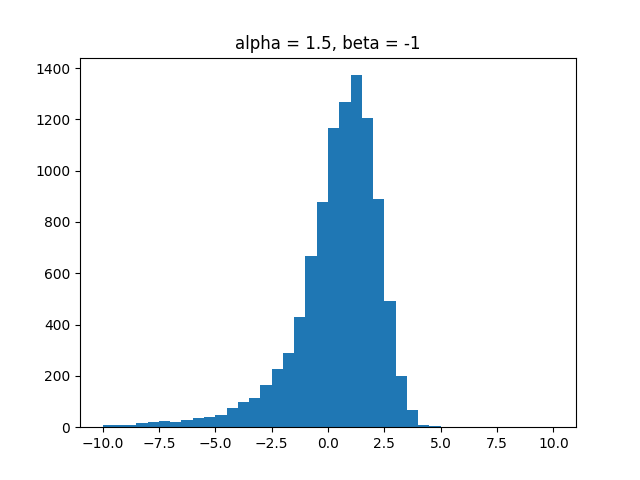
\includegraphics[width=\textwidth]{q4_1_a1.5_bn1}
    \end{minipage}%
    \begin{minipage}{0.2\textwidth}
        \centering
        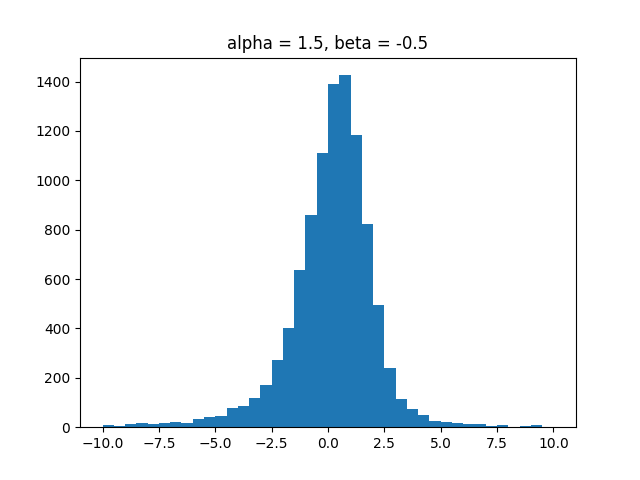
\includegraphics[width=\textwidth]{q4_1_a1.5_bn0.5}
    \end{minipage}%
    \begin{minipage}{0.2\textwidth}
        \centering
        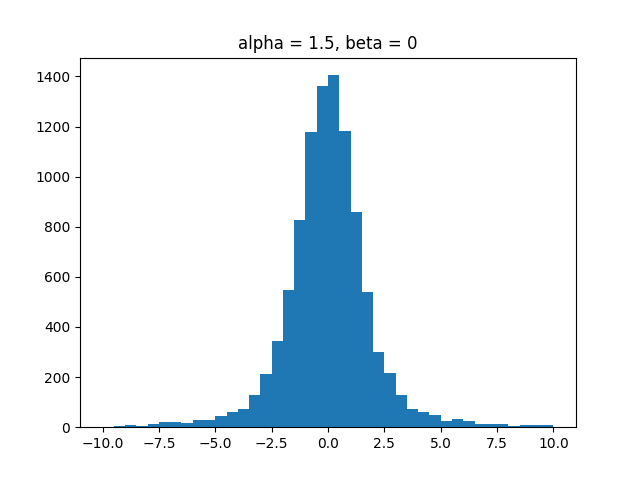
\includegraphics[width=\textwidth]{q4_1_a1.5_b0}
    \end{minipage}%
    \begin{minipage}{0.2\textwidth}
        \centering
        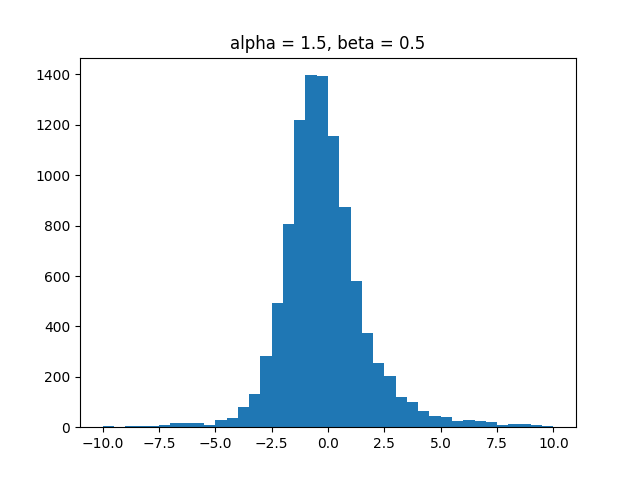
\includegraphics[width=\textwidth]{q4_1_a1.5_b0.5}
    \end{minipage}%
    \begin{minipage}{0.2\textwidth}
        \centering
        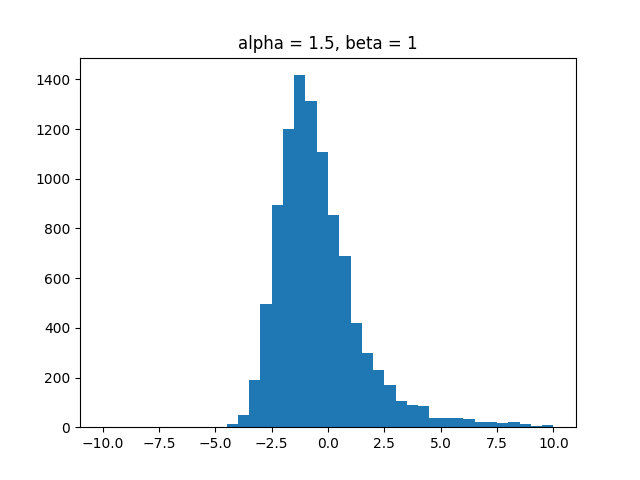
\includegraphics[width=\textwidth]{q4_1_a1.5_b1}
    \end{minipage}
    
    \caption{Histogram of sampled RV $X$ for different values of $\alpha$ and $\beta$}
    \label{fig:q4_1}
\end{figure*}

\subsection{Simulation for complex RV distributions}
\subsubsection{Generation of complex RV by sampling}

One strength of using the sampling method to generate RV is that it allows construction of RV with complex density distributions, where a general density function would be hard to calculate using methods including the Jacobian formula.

For a certain RV $X$ that is defined as:

\begin{flalign*}
    & \alpha \in (0,2) (a\neq 1), \beta \in [-1, +1] \\
    & b=\frac{1}{a}tan^{-1}(\beta tan(\pi \alpha/2)) \\
    & s=(1+\beta^2 tan^2(\pi \alpha/a))^{\frac{1}{2 \alpha}} \\
    & \text{Generate RVs: } U \sim \mathcal{U}(-\pi /2, +\pi /2) \\
    &                       V \sim \mathcal{E}(1) \\
    & X = s \frac{sin(\alpha(U+b))}{(cos(U))^{1/a}}(\frac{cos(U-\alpha(U+b))}{V})^{\frac{1-\alpha}{\alpha}} \\
\end{flalign*}

Fig~\ref{fig:q4_1} shows histogram plots of the RV $X$ when different values of the parameters $\alpha$ and $\beta$ are chosen. Each figure is produced using sample size $N=10000$ and 40 bins, each of width 0.5cm, which is tested to give an optimal demonstration of the density distribution.

Comparing the plots obtained for $\alpha=0.5$(first row) and $\alpha=1.5$(second row), it is observed that when $\alpha$ increase, the distribution becomes fuller and less steep, while a lower $\alpha$ value like 0.5 results in a sharp density peak centered around 0. Therefore $\alpha$ is likely to contribute to the spread of the distribution, and a higher $\alpha$ value gives a lower kurtosis.

Comparing the plots obtained for different values of $\beta$ that spread across the given permitted range of it, with $\alpha$ fixed, it is observed that $\beta$ controls the skewness of the sampled distribution. 

A negative $\beta$ value results in a negatively-skewed distribution where the median is left of the mode(peak of histogram), and a positive $\beta$ value results in a positive skew where the median is on the right of the mode. At $\beta=0$, the sampled distribution of $x$ appears to be almost symmetrical around 0.0.

\subsubsection{Tail probability for the complex distribution}
The tail probability of $X$ that $P(|X|>t)$ can be calculated as:

\begin{align*}
    P(|X|>t) &= P(X>t) + P(X<-t) \\
             &= (1-P(X<t)) + P(X<-t) \\
             &= 1-F(t)+F(-t)
\end{align*}

In terms of the distribution of $X$ generated by sampling described in the last section, this tail probability can also be approximated to the sum of histogram count data of samples outside the tail boundary.
When $\beta$ is fixed at 0, this would result in the tail probability as follows for $\alpha=0.5$ and $\alpha=1.5$ at tail boundaries $t=0, 3, 6$ (with reference to tail probabilities of a standard normal distribution):

\begin{table}[h!]
    \centering
    \begin{tabular}{|c|c|c|c|}
        \hline
        & t=0 & t=3 & t=6  \\ 
        \hline
        $\alpha=0.5$ & 1 & 0.3674 & 0.2768 \\ 
        $\alpha=1.5$ & 1 & 0.1032 & 0.03129 \\ 
        $\mathcal{N}(0,1)$ & 1 & 0.0027 & $1.973e^{-9}$ \\
        \hline
    \end{tabular}
    \caption{Tail probabilities of $X$ at different parameter combinations and standard normal}
    \label{table:q4_2}
\end{table}

As shown in Table~\ref{table:q4_2}, the tail probability of $X$ for both $\alpha$ settings is much higher than that of a standard normal distribution, which indicates that $X$ converges slower and hence is more spread-out than the standard normal. 
Additionaly, the $\alpha=1.5$ distribution has a significantly reduced tail probability than $\alpha=0.5$, which agrees with the graphical representations as the density distribution becomes wider yet more concentrated around 0 as $\alpha$ increases.

\begin{figure}[h]
    \centering
    \subfigure[$\alpha=0.5, \beta=0$]{
        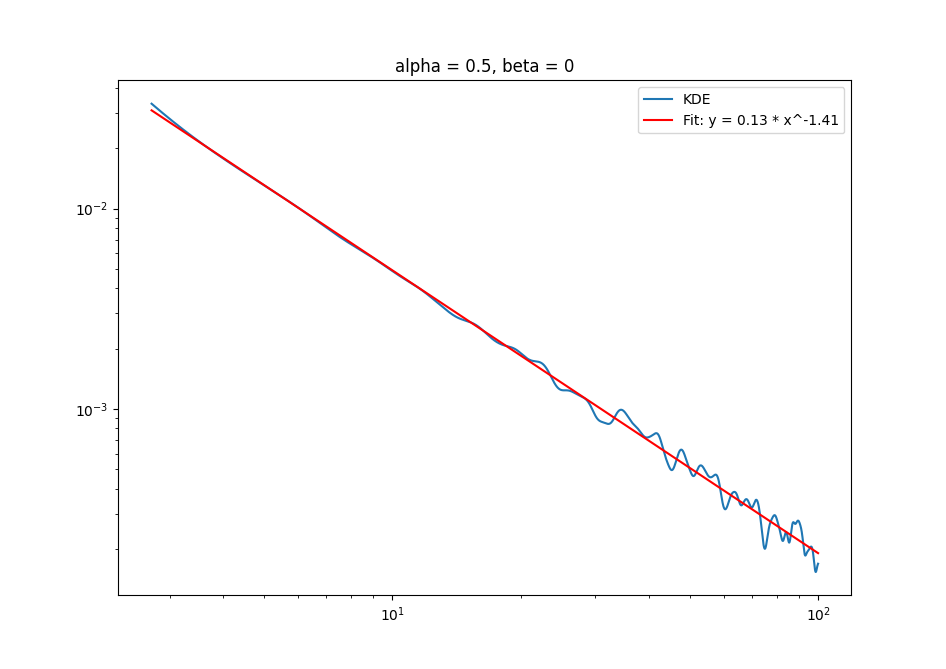
\includegraphics[width=0.5\textwidth, height=4.5cm]{q4_2_a0.5_80000_linreg}
        \label{fig:q4_2_a0.5_80000_linreg}
    }

    \subfigure[$\alpha=1.5, \beta=0$]{
        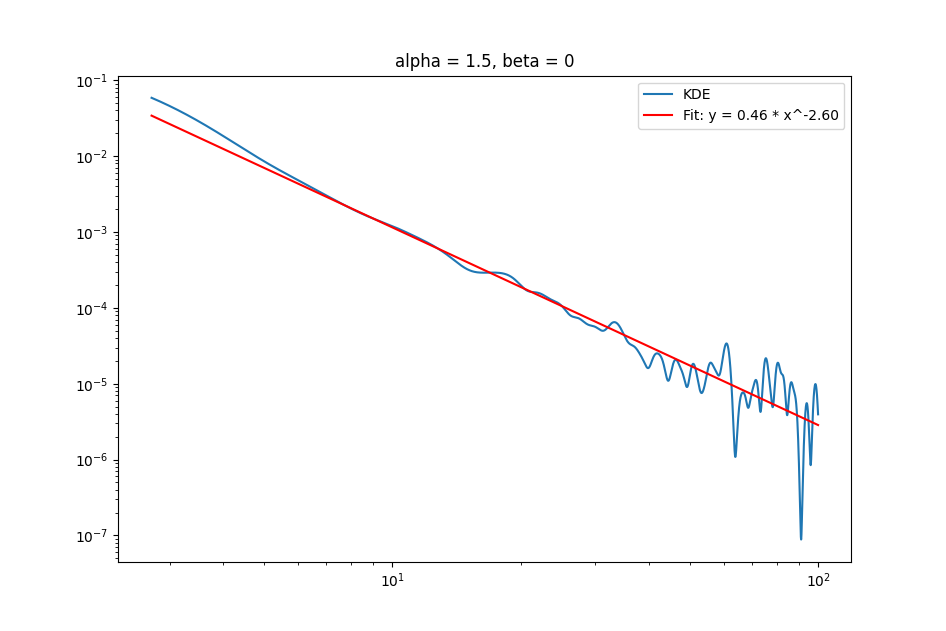
\includegraphics[width=0.5\textwidth, height=4.5cm]{q4_2_a1.5_80000_linreg}
        \label{fig:q4_2_a1.5_80000_linreg}
    }
    \caption{Tail probability of $X$ and linear regression fittings (sample size 80000; log-log)}
    \label{fig:q4_2_linreg}
\end{figure}

From closer observation of the distribution as sample size $N$ get large, it can be suspected that for large tail boundary $|x|$, the pdf can be approximated by a power expression $p(x)\approx cx^\gamma$, where $c$ and $\gamma$ are constants.
This relationship is better depicted as a log-log equation $log(p(x))=log(c) +\gamma log(x)$, which means $log(c)$ and $\gamma$ can be obtained as y-intercept and slope of the graph in log-log scale.

Experimenting with $\alpha=0.5$ or $\alpha=1.5$, at $\beta=0$, it is shown in Fig~\ref{fig:q4_2_linreg} that $c$ is relatively stable around 0.15. When repeating the regression fitting for other $\alpha$ values in the permitted range, it is concluded that $\gamma$ is related to $\alpha$ as $\gamma = -0.128\alpha - 0.077$.

\subsubsection{Relating $X$ with Gaussian distribution}
\begin{figure}[h]
    \centering
    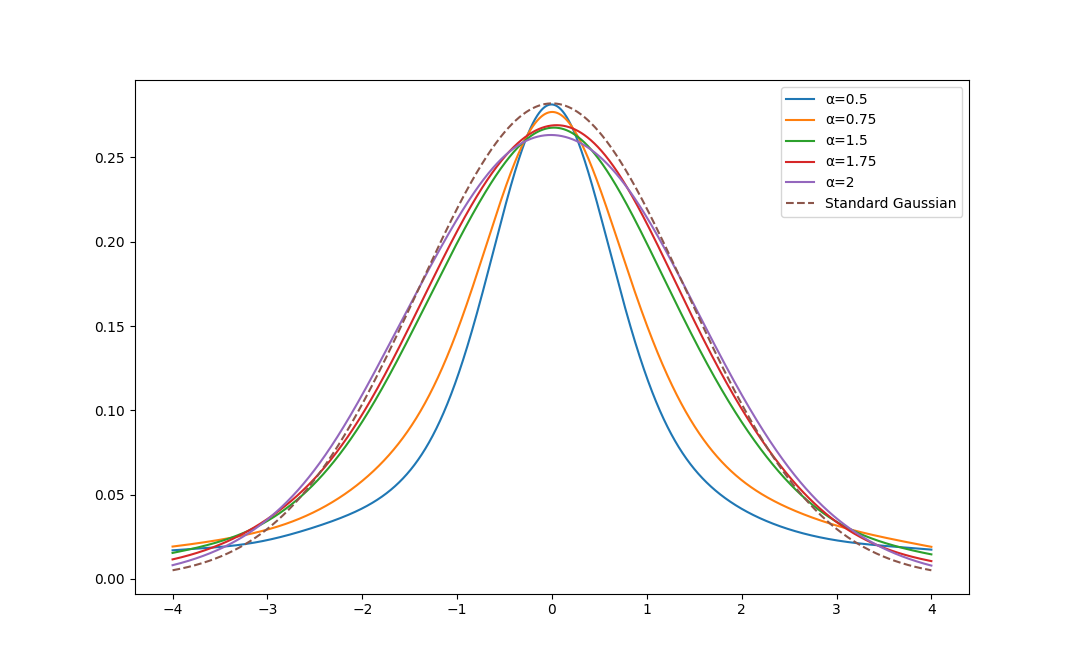
\includegraphics[width=0.53\textwidth, height=6cm]{q4_3}
    \caption{$X$ at different values of $\alpha$ compared to gaussian}
    \label{fig:q4_3}
\end{figure}

As shown in Fig~\ref{fig:q4_3}, the distribution of $X$ approaches that of Gaussina distribution with variance 2 $\mathcal{N}(0,2)$ as $\alpha$ get closer to 2.
This result aligns with the $\alpha =2$ special case of the stable distribution.

\section{Conclusion}
In this report, the investigations on applying Python programming to statistics of RV is explored, with a focus on data visualization using histograms and KDE, and generation of specific RV distributions using various methods including the Jacobian formula and inverse CDF methods. 
The capabilities of generating distributions through sampling is also discussed in detail, providing a better understanding of some of the properties of the stable diffusion.
Manipulations of sampled data including Monte Carlo estimates of mean and variance and tail probability calculations is investigated in this lab exercise, which prove to be useful tools that can transfer to other statistical applicaitons.

In conclusion, generating and presenting RV distributions using the above discussed methods and transformations contains great potentials and is expected to employ wide usage, as it makes scientific and engineering investigations efficient and accurate. Further explorations on this topic remains open as examining more complex and advanced methods would strengthen understanding of this profound area.

\end{document}